\documentclass[a4paper]{article}
\usepackage{graphicx}
\usepackage[utf8]{inputenc}
\usepackage[english, serbian]{babel}

\title{UseCase: Odabir prihvaćenih radova za tekuće izdanje časopisa}
\date{10.11.2018.}
\author{Dimitrije}

\begin{document}

\maketitle

\begin{itemize}
    \item Akter: Korisnik informacionog sistema
    \item Kratak opis: Korisnik informacionog sistema vrši pregled prethodnog izdanja časopisa.
    \item Osnovni tok događaja:
        \begin{enumerate}
            \item Korisnik zahteva od sistema pregled spisak prethodnih izdanja časopisa.
            \item Sistem prikazuje spisak prethodnih izdanja.
            \item Korisnik bira izdanje koje želi da pregleda.
            \item Sistem mu prikazuje traženo izdanje časopisa.
        \end{enumerate}
    \item Alternativni tok događaja:
        \begin{enumerate}
            \item  (2) Sistem ne prikazuje spisak prethodnih izdanja. Korisnik pokušava ponovo da izvrši korak 1. Ukoliko ne uspe, obraća se administratoru časopisa.
            \item (4) Sistem ne prikazuje traženo izdanje časopisa. Korisnik pokušava ponovo da izvrši korak 3. i eventualno menja izdanje koje želi da pregleda. Ukoliko korak 4. ne uspe, obraća se administratoru časopisa.
        \end{enumerate}
\end{itemize}

\begin{figure}
    \centering
    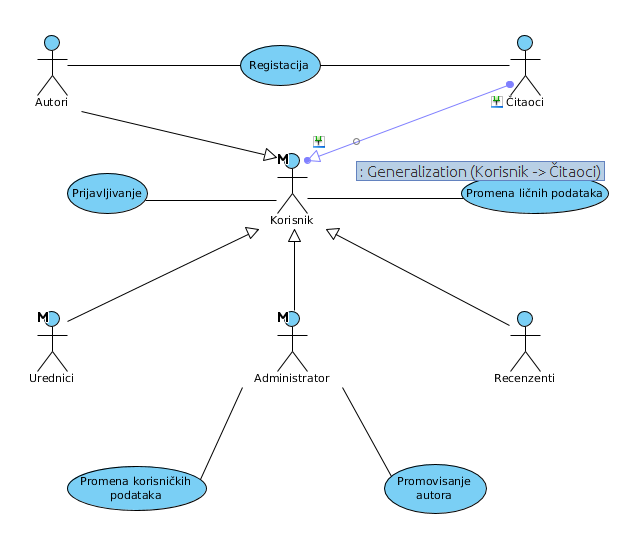
\includegraphics[width=\linewidth]{usecasePrijavljivanje.png}
    \caption{UseCase screenshot}
    \label{fig:my_label}
\end{figure}


\end{document}
